\section{Active Shape Model}

Active shape models are statistical models of the shape
of objects which iteratively deform to fit to an example
of the object in a new image.

\subsection{Load data}
For this assignment we are provided by a set of landmarks, each one
containing a list of points corresponding with the shape of a tooth.
Those landmarks should be used to build an Active shape model.
The first step is to load the landmarks. They are stored in list form,
following the format ${[X_1, Y_1, \ldots, X_n, Y_n]}^T$. To increase
the number of samples, the mirrored version of the landmarks is also
loaded.

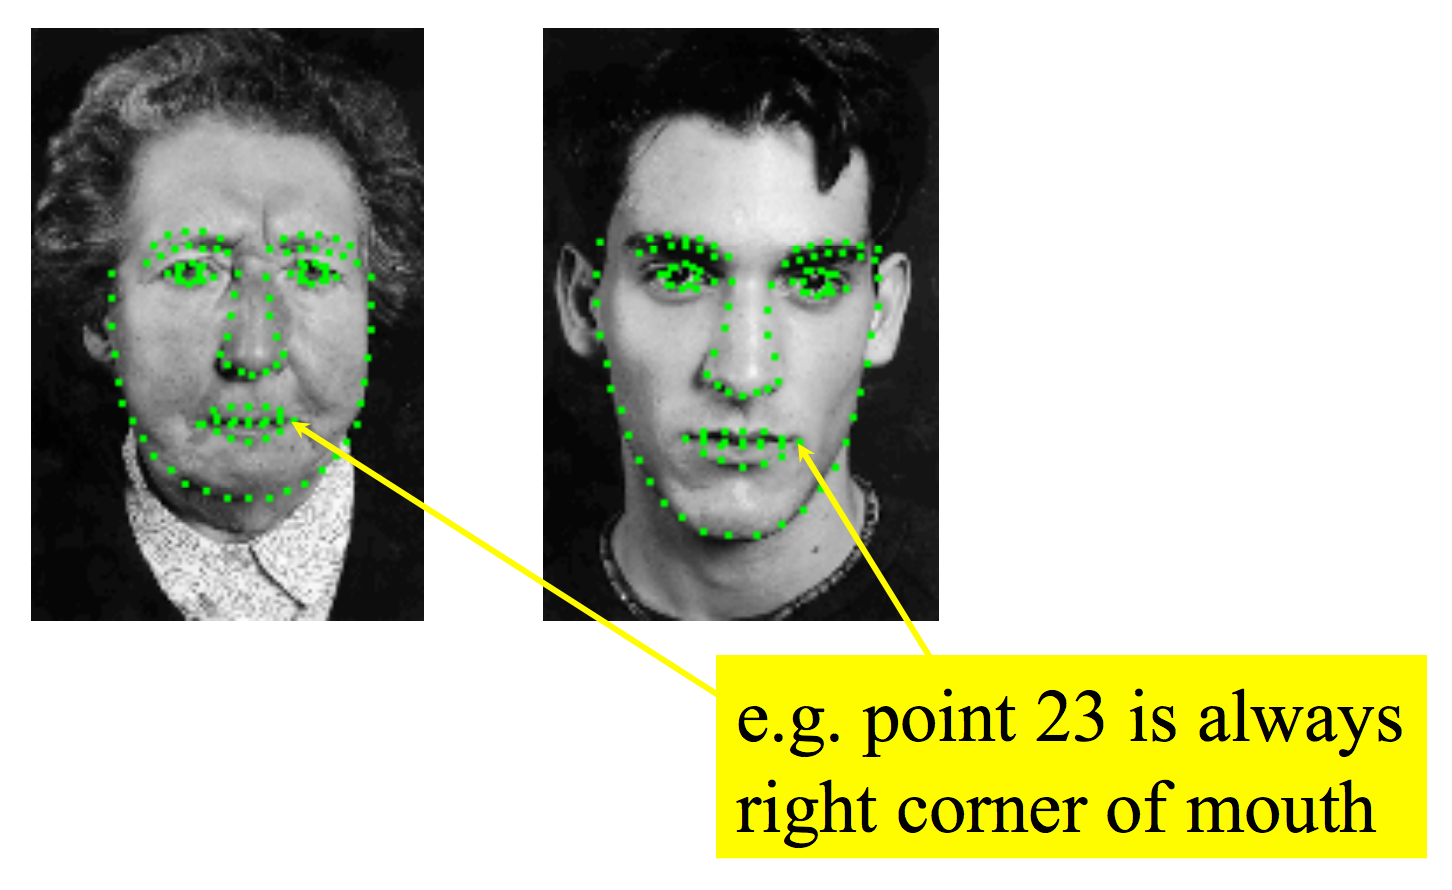
\includegraphics[width=0.7\linewidth]{img/landmarks}


\subsection{Align the training set}
% Procrustes Analysis
Once the landmarks are loaded, the training set must be aligned in
order to compare equivalent points from different shapes. This
alignment is done by scaling, rotating and translating the training
shapes using the following algorithm:

\begin{algorithm}
\SetAlgoLined 
Rotate, scale and translate each shape to align with the
first shape in the set\;
 \While{process has not converged}{
  Calculate the mean shape from the aligned shapes\;
  Normalize the orientation, scale and origin of the
  current mean to suitable defaults\;
  Realign every shape with the current mean\;
}
\caption{Procrustes Analysis}
\end{algorithm}

% image of the shapes before and after procrustes  


\subsection{Principal Component Analysis}
The set of aligned shapes contains as much dimensions as landmarks
have each shape. To reduce the dimensionality of the dataset and
get rid of the extra dimensions, Principal Component Analysis is
applied. It uses an orthogonal transformation to convert a set of
observations of possibly correlated variables into a set of values
of linearly uncorrelated variables called principal components.
The first principal component has the largest possible variance
and each succeeding component in turn has the highest variance
possible under the constraint that it is orthogonal to the
preceding components.

The first 8 components hold more than 98\% of variance. The
dimension of the dataset is reduced from 80 to 8.

% 8 dims - 98.6571035 variance
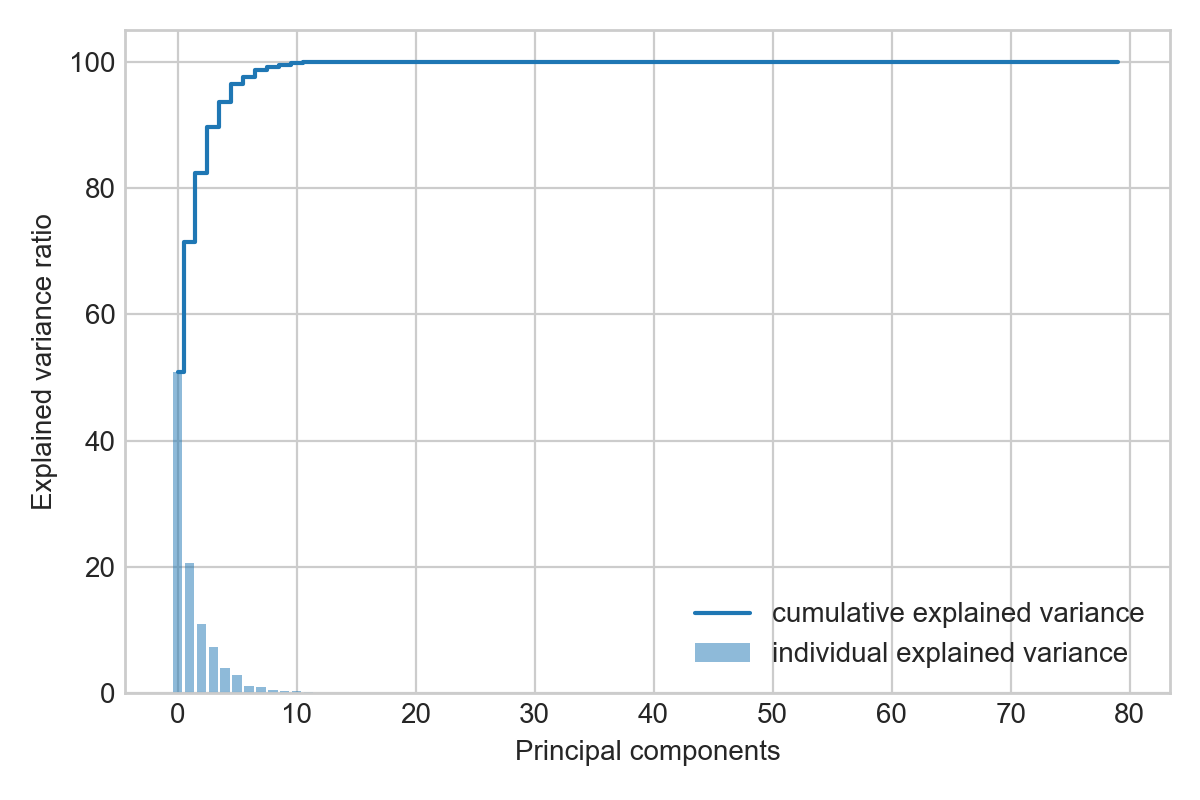
\includegraphics[width=0.7\linewidth]{img/variance}
